\documentclass[12pt,a4paper]{report}
% Preamble
\usepackage[T1]{fontenc}
\usepackage{lmodern}
\usepackage[top=1in,bottom=1in,left=1.1in,right=1.1in]{geometry}
\usepackage{hyperref}
\usepackage{dialogue}
% math packages
\usepackage{amsmath}
\usepackage{amssymb}
\usepackage{amsthm}
\usepackage{float}

% graphics and tables
\usepackage{graphicx}
\usepackage{booktabs}

% Code and algo
\usepackage{listings}
\usepackage{algorithm2e}

% --- UPGRADES ---
\usepackage{microtype}        % better justification, no rivers
\usepackage{xcolor}           % color support
\usepackage{enumitem}         % tighter list spacing
\usepackage{titlesec}         % section rule
\usepackage{fancyhdr}         % headers and footers
\usepackage{setspace}         % line spacing control
% ----------------
\usepackage{fontenc}
\usepackage{inputenc}
\RestyleAlgo{boxed}

\hypersetup{
    colorlinks=false,
    linkcolor=blue,
    urlcolor=blue,
    bookmarks=true,
}

\newcommand{\divline}{
    \vspace{1em}
    \begin{center}
        \rule{0.8\textwidth}{0.6pt}
    \end{center}
    \vspace{1em}
}


\newtheorem{definition}{Definition}
% --- Gray background for code (prints cleanly in B&W) ---
\lstset{
    language=Python,
    basicstyle=\ttfamily\small,
    keywordstyle=\bfseries,
    commentstyle=\itshape\color{gray},
    stringstyle=\color{gray!60!black},
    backgroundcolor=\color{gray!10},
    breaklines=true,
    frame=single,
    framesep=4pt,
    xleftmargin=6pt,
    xrightmargin=6pt,
    showstringspaces=false,
    numbers=left,
    numberstyle=\ttfamily\color{gray}
}
% --- List spacing ---
\setlist{itemsep=2pt, topsep=4pt, parsep=0pt}


% --- Section rule (default sizes, just adds a rule under \section) ---
\titleformat{\section}{\normalfont\Large\bfseries}{\thesection}{1em}{}[\titlerule]


\pagestyle{fancy}
\fancyhf{}
\renewcommand{\headrulewidth}{0.4pt}
\renewcommand{\footrulewidth}{0.4pt}
\fancyhead[L]{\small\textit{Artificial Intelligence and Applications}}
\fancyhead[R]{\small\textit{Sree Saicharan Vadapalli --- ET23BTIT133}}
\fancyfoot[C]{\small\thepage}

% Plain style for chapter-opening pages
\fancypagestyle{plain}{
  \fancyhf{}
  \renewcommand{\headrulewidth}{0pt}
  \renewcommand{\footrulewidth}{0.4pt}
  \fancyfoot[C]{\small\thepage}
}

% --- Line spacing ---
\setstretch{1.15}

\begin{document}

\title{\Huge Artificial Intelligence and Applications \\ Lab Practical File}
\author{\Large Sree Saicharan Vadapalli \\ Information Technology \\ ET23BTIT133}
\date{\today}
\maketitle
\newpage

\tableofcontents
\newpage
\renewcommand{\chaptername}{Practical}

\chapter{Analysis of Major AI Projects}
\section{Deep Blue}
In May 1997, IBM's Deep Blue, a chess-playing supercomputer designed by Feng-hsiung Hsu, defeated the reigning world chess champion Garry Kasparov under standard tournament controls. It was the first computer to win a game and a match against a reigning world champion. Deep Blue heavily relied on \textbf{game-tree search} and hand-made evaluation heuristics instead of modern machine learning techniques.

\subsection{Algorithmic Design and Evaluation Strategy}
Unlike modern learning-based systems, Deep Blue relied on deterministic search and expert-designed heuristics. It derived its strength primarily from a large and complex game-tree search combined with a handcrafted evaluation function.

\subsubsection{Tree Search}
A chess game can be represented as a tree search problem because it is deterministic, has perfect information and is zero-sum. Nodes represent alternating white and black positions and directed edges represent possible moves.

\subsubsection{Evaluation Function}
The evaluation function takes the current state of the game and reduces it to an estimated scalar value used for evaluating that state.
\[
\text{Score} = \sum_{i} w_i \, f_i(\text{position})
\]
where $f_i$ represents positional features and $w_i$ represents corresponding weights.

\subsubsection{Minimax and Alpha-Beta Pruning}
Deep Blue implemented a minimax search framework for deterministic, zero-sum, perfect-information games. The maximizing player selects moves to maximize the evaluation score while the minimizing player selects moves to minimize it. The formal recursive definition is:
\[
V(s) =
\begin{cases}
\text{Utility}(s) & \text{if } s \text{ is terminal} \\
\max\limits_{a \in \text{Actions}(s)} V(\text{Result}(s,a)) & \text{if } s \text{ is Max node} \\
\min\limits_{a \in \text{Actions}(s)} V(\text{Result}(s,a)) & \text{if } s \text{ is Min node}
\end{cases}
\]
The time complexity of minimax is $O(b^d)$ where $b$ is the branching factor and $d$ is the search depth.
With alpha-beta pruning, this reduces to $O(b^{d/2})$ in the best case, effectively doubling the searchable depth.
Alpha-beta pruning maintains two bounds: \textbf{Alpha $(\alpha)$}, the best value for the maximizing player, and \textbf{Beta $(\beta)$}, the best value for the minimizing player. A branch is pruned when $\alpha \ge \beta$.

\subsubsection{Transposition Tables}
Deep Blue used transposition tables with Zobrist hashing to store previously evaluated positions, allowing constant-time lookup and avoiding redundant computation.

\subsection{System Architecture}
The 1997 version of Deep Blue consisted of 30 IBM RS/6000 SP nodes, 480 custom VLSI chess chips, and high-speed interconnects for distributed computation. Each node had custom chess processors capable of generating legal moves in hardware and performing search acceleration. It implemented root-level parallelism through a master-slave architecture, where different processors explored different legal moves simultaneously.

\subsection{Performance, Limitations and Impact}
Deep Blue evaluated 200 million positions per second and searched to depths of six to eight moves, up to twenty in tactical lines. Despite its success, it was a specialized system with no learning capability, a manually engineered evaluation function, and a dependence on domain-specific hardware. Its victory over Kasparov demonstrated that large-scale computational search could surpass human expertise, influencing later systems such as AlphaZero.

\section{Chinook}
Chinook is a computer checkers program developed at the University of Alberta under Jonathan Schaeffer. It defeated reigning world checkers champion Marion Tinsley, and by 2007 the team had weakly solved the game of checkers, proving that perfect play from both sides results in a draw.

\subsection{Computational Characteristics of English Draughts}
English draughts is a deterministic, perfect-information, two-player zero-sum game. The entire game can be represented as a finite directed graph where nodes are legal positions, edges are legal moves, and terminal nodes denote win, loss, or draw. Key state space metrics are:
\begin{itemize}
    \item Estimated total legal positions $\approx 10^{20}$
    \item Average branching factor $\approx 8$--$10$ moves per position
    \item Maximum game length bounded by repetition and capture rules
\end{itemize}
A game is solvable if its state space can be fully enumerated, terminal outcomes can be propagated backward, and storage and compute resources are sufficient. Checkers met these conditions far before chess or Go.

\subsection{Algorithmic Design and Evaluation Function}
Chinook used depth-limited minimax with alpha-beta pruning and iterative deepening, augmented by transposition tables indexed via Zobrist hashing. The evaluation function combined material balance, piece advancement, mobility, center control, and structural formations, refined through expert consultation rather than machine learning. In endgame scenarios, heuristic evaluation was replaced by exact lookup into precomputed databases generated through retrograde analysis. Retrograde analysis works backward from terminal positions, propagating values using:
\[
V(s) = \begin{cases} 1 & \text{if } s \text{ is a win} \\ 0 & \text{if } s \text{ is a draw} \\ -1 & \text{if } s \text{ is a loss} \end{cases}
\]

\subsection{Performance, Limitation and Impact}
Chinook consistently evaluated millions of positions per move and guaranteed optimal decisions in endgame positions via database lookup. It was however domain-specific and non-generalizable, requiring extensive precomputation and not scaling to larger games. Its 2007 weak solution of checkers was the first complete resolution of a non-trivial classical board game and influenced subsequent research in computational game theory and formal game solving.

\section{ALVINN}
In 1989, Dean Pomerleau at Carnegie Mellon University developed ALVINN (Autonomous Land Vehicle In a Neural Network), one of the earliest end-to-end neural network systems for autonomous driving. ALVINN learned steering control directly from camera images using supervised training, deployed on the Navlab research vehicle.

\subsection{Network Architecture and Learning Mechanism}
ALVINN consisted of a three-layer backpropagation neural network.

\subsubsection{Input Layer}
ALVINN processed $30\times32$ grayscale images flattened into a 960-dimensional vector, receiving data from cameras and laser range finders.

\subsubsection{Hidden Layer}
The hidden layer consisted of approximately 30 neurons, each connected to all 960 input nodes. During training it learned internal representations such as road boundaries, lane markings, and road texture without manually designed feature extraction.

\subsubsection{Output Layer}
The output layer consisted of 45 units, each representing a possible steering direction. The center unit signals straight ahead, with units to either side corresponding to progressively sharper turns. A hill-shaped activation centered on the correct unit indicated the curvature needed to reach the center of the road roughly 7 meters ahead.

\subsection{Performance, Limitations, and Impact}
ALVINN demonstrated sustained autonomous steering at speeds up to 55 mph over several kilometers. Its primary limitation was poor generalization to conditions not in the training data — it had no geometric or semantic understanding of the environment, controlled only steering, and operated on very low-resolution input. It was among the first systems to demonstrate end-to-end neural control of a real vehicle, directly influencing NVIDIA's DAVE and PilotNet decades later.

\section{ELIZA}
In 1966, Joseph Weizenbaum at MIT developed ELIZA, one of the earliest natural language processing programs. ELIZA operated by pattern matching user input against predefined script rules and reflecting the user's own statements back at them. Its most well-known script, \textbf{DOCTOR}, simulated a Rogerian psychotherapist. ELIZA possessed no understanding of language; its apparent intelligence was entirely an artifact of pattern substitution, a phenomenon Weizenbaum termed the \textit{ELIZA effect}.

\subsection{Algorithmic Design}

\subsubsection{Pattern Matching and Decomposition}
Each input sentence was scanned for keywords ranked by priority weight. Upon identifying the highest-priority keyword, ELIZA applied a decomposition rule that parsed the sentence into fragments using wildcard matching, then reassembled them into a response with simple pronoun substitution. If no keyword matched, ELIZA fell back to context-free defaults such as \textit{``Please go on''}.

\subsubsection{Script Architecture}
Rules were encoded in a separate interchangeable script file, allowing different conversational personas to be loaded by supplying a different script. The DOCTOR script contained approximately 200--250 decomposition and reassembly rules.

\subsection{Performance, Limitations, and Impact}
ELIZA produced coherent responses for short exchanges within the DOCTOR script but had no memory beyond the immediately preceding statement and could not maintain consistency across longer dialogues. It possessed no semantic understanding, relying entirely on syntactic pattern matching with no internal representation of meaning. ELIZA introduced the concept of a chatbot, and the ELIZA effect remains a relevant concern in the evaluation of modern large language models.

\section{ChatGPT}
In November 2022, OpenAI released ChatGPT, a large language model built on the GPT architecture, fine-tuned using Reinforcement Learning from Human Feedback (RLHF). It demonstrated unprecedented fluency across coding, writing, analysis, and question answering, reaching one million users within five days of launch.

\subsection{Architectural Design}

\subsubsection{Transformer Architecture}
ChatGPT is based on the decoder-only transformer architecture. The core mechanism is \textbf{scaled dot-product self-attention}, allowing every token to attend to every other token in the sequence. Multi-head attention runs this in parallel across multiple heads, capturing information from different representational subspaces simultaneously. The attention is computed as:
\[
\text{Attention}(Q, K, V) = \text{softmax}\!\left(\frac{QK^\top}{\sqrt{d_k}}\right)V
\]
where $Q$, $K$, $V$ are the query, key, and value matrices and $d_k$ is the key dimension.

\subsubsection{Pre-training Objective}
The model is trained on a \textbf{next-token prediction} objective over a large text corpus, forcing it to internalize syntactic, semantic, and factual structure without task-specific supervision. The objective minimizes the negative log-likelihood:
\[
\mathcal{L} = -\sum_{t=1}^{T} \log P(x_t \mid x_1, x_2, \ldots, x_{t-1})
\]

\subsubsection{Reinforcement Learning from Human Feedback}
After supervised fine-tuning, a reward model is trained on human preference rankings of model outputs. The language model is then optimized using Proximal Policy Optimization (PPO) to maximize the reward signal, with a penalty preventing excessive deviation from the supervised baseline.

\subsection{Performance, Limitations, and Impact}
ChatGPT demonstrated strong performance across code generation, mathematical reasoning, and multi-turn dialogue. GPT-4 achieved near-human performance on benchmarks including the bar exam and GRE. Its primary limitation is \textbf{hallucination} — generating factually incorrect statements confidently — along with sensitivity to prompt phrasing and bias inherited from training data. ChatGPT established RLHF as the dominant alignment technique and triggered rapid development of competing systems from Google, Meta, and Anthropic.

\section{Google Translate}
Google Translate is a multilingual machine translation service first launched in April 2006. It initially used statistical machine translation (SMT) and transitioned to a neural machine translation (NMT) architecture in 2016 with the Google Neural Machine Translation (GNMT) system.
\subsection{Algorithmic Design}

\subsubsection{Statistical Machine Translation}
The original SMT system modeled translation as a probabilistic search problem, finding the target sentence that maximized the product of a translation model and a language model, implemented as a log-linear combination of feature functions. It handled long-range syntactic dependencies poorly.

\subsubsection{Neural Machine Translation and Attention}
GNMT replaced the phrase-based pipeline with an encoder-decoder architecture. The encoder produces a sequence of hidden states; the decoder generates the target sequence one token at a time using an \textbf{attention mechanism} that computes a weighted sum over encoder hidden states. The attention weight for source token $j$ when generating target token $t$ is:
\[
\alpha_{t,j} = \frac{\exp(e_{t,j})}{\sum_{k=1}^{T} \exp(e_{t,k})}, \quad e_{t,j} = \text{score}(h_t, \bar{h}_j)
\]
where $h_t$ is the decoder hidden state and $\bar{h}_j$ is the encoder hidden state at position $j$. Modern Google Translate uses Transformer encoders and decoders for higher parallelism.

\subsection{Performance, Limitations, and Impact}
The transition from SMT to NMT reduced translation errors by approximately 60\% on several language pairs. Quality degrades for low-resource languages, idiomatic expressions, and languages with complex morphology. Google Translate substantially lowered the barrier to cross-lingual communication and demonstrated zero-shot translation, showing that neural networks could form language-agnostic semantic representations.

\section{Gemini}
In December 2023, Google DeepMind released Gemini, a family of natively multimodal large language models designed to reason across text, images, audio, video, and code within a unified architecture. It was released in three tiers: Ultra, Pro, and Nano.

\subsection{Architectural Design}

\subsubsection{Multimodal Architecture}
Gemini accepts interleaved token sequences from multiple modalities. Images and video are encoded via a learned visual encoder, audio via a learned audio encoder, and text via a subword tokenizer. All tokens are projected into a shared embedding space and processed jointly by the transformer decoder, enabling cross-modal attention within the same computation.

\subsubsection{Mixture of Experts}
Gemini 1.5 employs a \textbf{Mixture of Experts} (MoE) architecture where a learned gating function routes each token to only the top-$k$ most relevant expert networks. This allows a very large total parameter count while keeping per-token compute cost manageable, enabling the million-token context window in Gemini 1.5.

\subsection{Performance, Limitations, and Impact}
Gemini Ultra achieved state-of-the-art results on 30 of 32 benchmarks at release, including MMLU at 90.0\%. It is susceptible to hallucination and spatial reasoning errors, and inference cost for Ultra-scale models remains high. Gemini established natively multimodal training as a standard paradigm and demonstrated the practical viability of million-token context windows, influencing the design of subsequent large models across the industry.

\section{Nano Banana}
Nano Banana is an AI-powered image generation system by Bananas Inc., using a latent diffusion model conditioned on natural language prompts for high-quality, fast text-to-image synthesis targeting resource-efficient deployment.

\subsection{Algorithmic Design}

\subsubsection{Latent Diffusion Model}
Rather than diffusing in pixel space, an autoencoder compresses the image into a lower-dimensional latent representation and the diffusion process operates there. The forward diffusion process adds noise according to:
\[
q(z_t \mid z_0) = \mathcal{N}(z_t;\, \sqrt{\bar{\alpha}_t}\, z_0,\, (1 - \bar{\alpha}_t)I)
\]
The U-Net is trained to minimize the denoising loss:
\[
\mathcal{L} = \mathbb{E}_{z, \epsilon, t}\!\left[\|\epsilon - \epsilon_\theta(z_t, t, c)\|^2\right]
\]
where $\epsilon$ is the true noise, $\epsilon_\theta$ is the predicted noise, and $c$ is the text conditioning.

\subsubsection{Text Conditioning via Cross-Attention}
The text prompt is encoded into embeddings by a text encoder (CLIP or T5 variant). Cross-attention layers at each U-Net resolution level allow spatial feature maps to attend over the full prompt embedding, conditioning every denoising step on the complete text description.

\subsubsection{Efficient Inference}
Nano Banana uses \textbf{DDIM} sampling, reformulating the reverse process as a deterministic update rule allowing generation in 20--50 steps rather than the 1000 used during training. Model distillation and quantization further reduce memory requirements for on-device deployment.

\subsection{Performance, Limitations, and Impact}
Nano Banana produces images up to $1024\times1024$ pixels in 20--50 DDIM steps and supports negative prompting. It can produce anatomically incorrect outputs, struggles with precise spatial layout, and text rendering within images is unreliable. It contributes to democratizing image generation by demonstrating high-quality synthesis on consumer hardware, reflecting a broader trend toward accessible on-device generative AI.

\section{Conclusion}
The systems studied span decades of AI development, from rule-based search in Deep Blue and Chinook to end-to-end neural learning in ALVINN, and finally to large-scale transformer models in ChatGPT, Google Translate, and Gemini. Early systems achieved superhuman performance in narrow domains through exhaustive search and handcrafted heuristics, but could not generalize beyond their target problem. Neural approaches replaced explicit rules with learned representations, enabling broader generalization at the cost of interpretability. ELIZA, despite its simplicity, remains a cautionary example that fluent output does not imply understanding, a concern that persists in modern language models.
\\
\divline
\chapter{8 Puzzle Problem}

\section{Problem Statement}
Write a program to solve the 8-puzzle. First, check if the puzzle is solvable.
If solvable, starting from any input state, it should display the sequence of
moves to reach the ordered output state. Rule to move: Slide a tile from a
non-empty square to an adjoining empty square.

\medskip
\noindent\textbf{Example:}

\medskip
\noindent
\begin{tabular}{cc}
    \begin{tabular}{|c|c|c|}
        \hline
        1 & 2 & 4 \\
        \hline
        8 & 3 & 6 \\
        \hline
          & 7 & 5 \\
        \hline
    \end{tabular}
    &
    \begin{tabular}{|c|c|c|}
        \hline
        1 & 2 & 3 \\
        \hline
        4 & 5 & 6 \\
        \hline
        7 & 8 &   \\
        \hline
    \end{tabular}
    \\[6pt]
    \textbf{Input state} & \textbf{Output state}
\end{tabular}
\section{Theory}
The 8-puzzle is a classic combinatorial search problem consisting of a $3 \times 3$
grid containing eight numbered tiles and one blank square. The objective is to
reach a predefined goal arrangement by sliding tiles into the blank space one at
a time. It is one of the simplest instances of the general $n$-puzzle and has been
widely used as a benchmark for evaluating search algorithms.

\subsection{State Space Representation}
The 8-puzzle can be modeled as a state space search problem. Each unique
arrangement of tiles on the board represents a \textbf{state}, and each legal
tile slide represents a \textbf{transition} between states. The initial arrangement
is the start state and the ordered arrangement is the goal state. The problem
reduces to finding a path from the start state to the goal state in this space.
The total number of distinct states is $9! = 362880$, of which exactly half are
reachable from any given state.

\subsection{Solvability}
Not all initial configurations of the 8-puzzle are solvable. Solvability is
determined by counting \textbf{inversions} in the flattened tile sequence
(excluding the blank). An inversion is a pair of tiles $(a, b)$ such that $a$
appears before $b$ in the sequence but $a > b$. For a $3 \times 3$ grid with
the blank on an odd-width board, a configuration is solvable if and only if the
number of inversions is even.

\subsection{A* Search}
A* is an informed search algorithm that finds the shortest path from a start
state to a goal state by evaluating each state using the function:
\[
f(n) = g(n) + h(n)
\]
where $g(n)$ is the cost of reaching state $n$ from the start (number of moves
made so far) and $h(n)$ is a heuristic estimate of the cost to reach the goal
from $n$. A* is guaranteed to find the optimal solution provided the heuristic
is \textbf{admissible}, meaning it never overestimates the true cost. This
implementation uses \textbf{Manhattan distance} as the heuristic:
\[
h(n) = \sum_{i=1}^{8} \left( |r_i - r_i^*| + |c_i - c_i^*| \right)
\]
% \section{Algorithm}
% \begin{algorithm}[H]
% \caption{8-Puzzle Solver using A* Search}
% \KwIn{Initial board state, Goal board state}
% \KwOut{Sequence of moves to reach the goal state, or infeasible message}

% Check solvability by counting inversions in the initial state\;
% \If{inversion count is odd}{
%     \Return{Puzzle is not solvable}\;
% }
% Initialize open list (priority queue) with the initial state\;
% Initialize closed list as empty\;
% \While{open list is not empty}{
%     Pop state with lowest $f = g + h$ from open list\;
%     \If{current state == goal state}{
%         Trace back path and \Return{sequence of moves}\;
%     }
%     Add current state to closed list\;
%     \ForEach{valid neighbor of current state}{
%         \If{neighbor not in closed list}{
%             Compute $g$ (moves so far) and $h$ (Manhattan distance to goal)\;
%             Push neighbor onto open list\;
%         }
%     }
% }
% \Return{No solution found}\;
% \end{algorithm}
\section{Implementation}
This practical implements the 8 puzzle problem in Python programming language using the A* algorithm.
\begin{lstlisting}
import heapq

GOAL = [[1,2,3],[4,5,6],[7,8,0]]

def is_solvable(state):
    flat = [n for row in state for n in row if n != 0]
    inversions = sum(1 for i in range(len(flat)) for j in range(i+1, len(flat)) if flat[i] > flat[j])
    return inversions % 2 == 0

def manhattan(state):
    dist = 0
    for i in range(3):
        for j in range(3):
            v = state[i][j]
            if v != 0:
                dist += abs(i - (v-1)//3) + abs(j - (v-1)%3)
    return dist

def neighbors(state):
    result = []
    flat = [n for row in state for n in row]
    r, c = divmod(flat.index(0), 3)
    for dr, dc, move in [(-1,0,'Up'),(1,0,'Down'),(0,-1,'Left'),(0,1,'Right')]:
        nr, nc = r+dr, c+dc
        if 0 <= nr < 3 and 0 <= nc < 3:
            s = [row[:] for row in state]
            s[r][c], s[nr][nc] = s[nr][nc], s[r][c]
            result.append((s, move))
    return result

def solve(start):
    if not is_solvable(start):
        return 'Not solvable'
    heap = [(manhattan(start), 0, start, [])]
    visited = set()
    while heap:
        _, g, state, path = heapq.heappop(heap)
        key = tuple(n for row in state for n in row)
        if key in visited:
            continue
        visited.add(key)
        if state == GOAL:
            return path
        for s, move in neighbors(state):
            if tuple(n for row in s for n in row) not in visited:
                heapq.heappush(heap, (g+1+manhattan(s), g+1, s, path+[move]))
    return 'No solution found'

start = [[1,2,4],[8,3,6],[0,7,5]]
result = solve(start)
print('Moves:', ' -> '.join(result) if isinstance(result, list) else result)
print('Total moves:', len(result) if isinstance(result, list) else '-')
\end{lstlisting}
\section{Output}
\begin{figure}[H]
    \centering
    \fbox{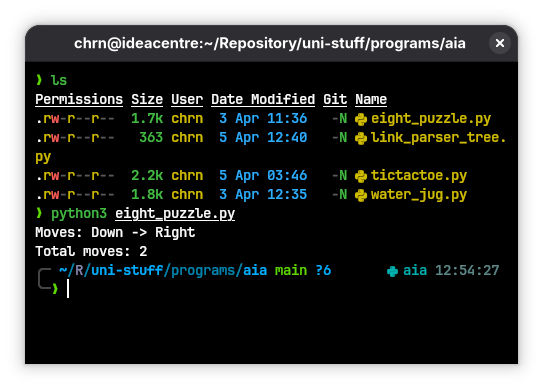
\includegraphics[width=0.8\linewidth]{attachments/eight_puzzle.png}}
    \caption{Output of the 8-Puzzle solver}
\end{figure}
\section{Conclusion}
In this practical, the 8-puzzle problem was successfully implemented using the A*
search algorithm with Manhattan distance as the heuristic. This practical demonstrates
how informed search strategies can effectively solve combinatorial puzzles.
\\
\divline
\chapter{Water Jug Problem}

\section{Problem Statement}
Implement the Water Jug Problem. The state of the system is represented as $(x,y)$ where $x$
is the quantity of water in the $4\hspace{0.3em} gallon$ jug and $y$ is the quantity of water in the
$3\hspace{0.3em} gallon$ jug. Assume the initial state to be $(0,0)$ and the goal state to be $(2,0)$.
Output the sequence of steps to go from the initial to the goal state.

\section{Theory}
The water jug problem is a classic \textbf{state-space search problem}. It consists of two jugs
with capacities of $4\hspace{0.3em} gallons$ and $3\hspace{0.3em} gallons$ respectively. The water
supply is assumed to be unlimited for the sake of simplicity. The goal state requires exactly $2 \hspace{0.3em} gallons$
of water in the $4 \hspace{0.3em} gallon$ jar and the $3 \hspace{0.3em} gallon$ jar must be empty.

\subsection{State Representation}
Each state in the system is represented as an ordered pair $(x,y)$, where:

\begin{itemize}
        \item $x = \text{amount of water in the 4-gallon jug}$
        \item $y = \text{amount of water in the 2-gallon jug}$
        \item $Initial \; State = (0,0)$
        \item $Goal \; State = (2,0)$
\end{itemize}

\subsection{Allowed Operations}
\begin{table}[H]
    \centering
    \begin{tabular}{@{}ll@{}}
    \toprule
    \textbf{Operation} & \textbf{Description} \\
    \midrule
    Fill 4-gallon jug   & Set $x = 4$ \\
    Fill 3-gallon jug   & Set $y = 3$ \\
    Empty 4-gallon jug  & Set $x = 0$ \\
    Empty 3-gallon jug  & Set $y = 0$ \\
    Pour 4 $\to$ 3      & Transfer until 3 is full or 4 is empty \\
    Pour 3 $\to$ 4      & Transfer until 4 is full or 3 is empty \\
    \bottomrule
    \end{tabular}
    \caption{Allowed operations in the Water Jug Problem}
\end{table}
These operations can be performed in any given state of the water jug problem.

\subsection{Search Approach}
Uninformed search strategies such as BFS (Breadth-First Search) and DFS (Depth-First Search) can be used to explore the state space search.
However, \textbf{BFS guarantees the shortest sequence of operations to reach the goal state}.
The search comes to a halt when the goal state is reached.

\subsubsection{Breadth-First Search Algorithm}
This algorithm explores all the states at the \textbf{current depth level} before moving to the
next level, guaranteeing the shortest path to the goal. For the water jug problem, BFS systematically
applies all six operations from each state ensuring minimum number of steps to reach the goal state.


\subsection{Problem Characteristics}
The water jug problem has the following characteristics:
\begin{itemize}
    \item Water jug problem has a \textbf{finite state space} as the maximum possible states are $5 \times 4 = 20$
    \item Each operation produces a unique new state, making the problem \textbf{deterministic}
    \item Exhaustive search can be safely used as the problem's state space is small.
\end{itemize}

\section{Implementation}
This practical has been implemented using the Best-First-Search (BFS) algorithm in the Python programming langauge.
\begin{lstlisting}
from collections import deque

def solve_water_jug():
    queue = deque()
    queue.append((start, [start]))
    visited = set()
    visited.add(start)
    while queue:
        (x, y), path = queue.popleft()

        if (x, y) == goal:
            print("Solution found!")
            print(f"Total steps: {len(path) - 1}")
            print("\nSequence of states:")
            for i, state in enumerate(path):
                print(f"Step {i}: ({state[0]}, {state[1]})")
            return path

        next_states = []
        next_states.append((4, y))
        next_states.append((x, 3))
        next_states.append((0, y))
        next_states.append((x, 0))
        pour = min(x, 3 - y)
        next_states.append((x - pour, y + pour))

        pour = min(y, 4 - x)
        next_states.append((x + pour, y - pour))
        for new_state in next_states:
            if new_state not in visited:
                visited.add(new_state)
                queue.append((new_state, path + [new_state]))

    print("No solution found!")
    return None

if __name__ == "__main__":
    solve_water_jug()
\end{lstlisting}

\section{Output}
\begin{figure}[H]
    \centering
    \fbox{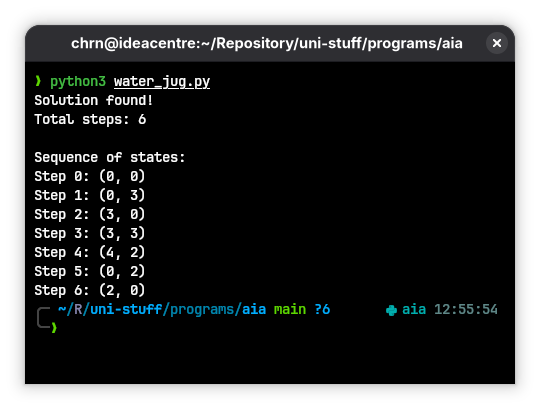
\includegraphics[width=0.8\linewidth]{attachments/water_jug.png}}
    \caption{Output of water jug problem solver}
\end{figure}

\section{Conclusion}
In this practical, the water jug problem was successfully implemented using the BFS
algorithm. This practical demonstrates the capability of uninformed search strategies
in solving the water jug problem.
\\
\divline

% TODO
\chapter{Basic Medical Expert System in Prolog}
\section{Problem Statement}
Develop an Expert System for medical diagnosis in Prolog. Given the symptoms, the expert system
should predict the disease; given the disease, the expert system should display the symptoms.

\section{Theory}
\subsection{Expert Systems}
It encodes human expertise as a set of rules and applies it to a collection of known facts to draw conclusions.
Modern expert systems include [[Machine Learning]] to enable the system to learn from its experiences.
The expert knowledge must be obtained from human experts or other sources like text, journals, articles, etc.
Expert systems separate "what is known?" from "How to reason about it?".

\begin{definition}
Expert Systems are AI systems that emulates decision-making of a human expert to solve complex problems in a specific domain.
\end{definition}

\subsubsection{Features of an Expert System}
\begin{itemize}
\item The control program (inference engine) is completely decoupled from the knowledge it operates over (knowledge base). Therefore, knowledge can be incrementally added and modified in knowledge base without recompiling the control program.
\item Expert systems use knowledge as heuristics as opposed to concrete algorithms that reach a conclusion.
\item Expert system shell is an expert system that can be used with different knowledge bases producing different expert systems.
\item It has the capability to explain how it reached a particular conclusion.
\item It uses symbolic representation for knowledge and performs inference through symbolic computation.
\item Expert systems also reason using meta-knowledge.
\end{itemize}

\subsubsection{Core Components of an Expert System}
\begin{enumerate}
\item Knowledge Base
\item Fact Database
\item Inference Engine
\item Explanation Facility
\item Knowledge Acquisition Facility
\item User Interface
\end{enumerate}

\subsubsection{Expert Systems Flow Diagram}
\begin{figure}[H]
\centering
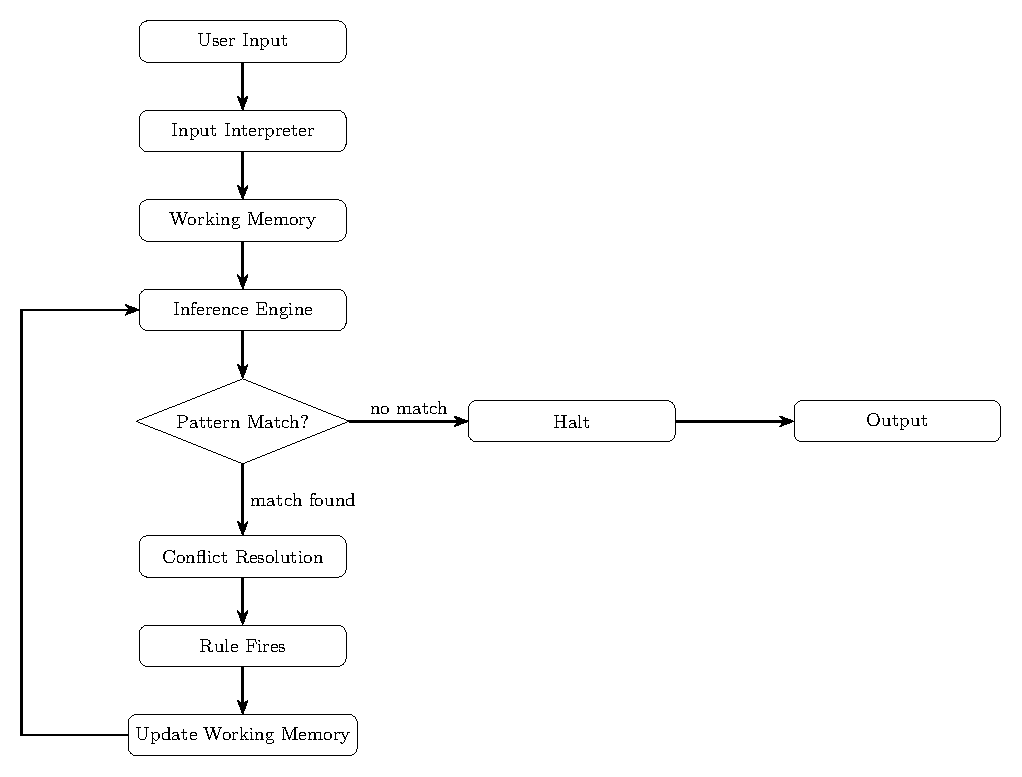
\includegraphics[width=1.0\linewidth]{attachments/expert_system.pdf}
\caption{Expert System Inference Cycle}
\end{figure}

\section{Implementation}
\begin{lstlisting}
domains
    disease = flu; cold; malaria.
    symptom = fever; cough; sneezing; headache.
    symptom_list = symptom*

predicates
    disease(disease, symptom_list)
    diagnose(symptom_list, disease)
    find_symptoms(disease, symptom_list)
    subset(symptom_list, symptom_list)
    member(symptom, symptom_list)

clauses
    disease(flu, [fever, cough]).
    disease(cold, [cough, sneezing]).
    disease(malaria, [fever, headache]).

    member(X, [X|_]).
    member(X, [_|T]) :- member(X, T).

    subset([], _).
    subset([H|T], L) :-
        member(H, L),
        subset(T, L).

   diagnose(Symptoms, Disease) :-
        disease(Disease, S),
        subset(Symptoms, S).

   find_symptoms(Disease, Symptoms) :-
        disease(Disease, Symptoms).
\end{lstlisting}

\section{Output}
\begin{lstlisting}
# OUTPUT
diagnose([fever,cough], D).
	D = flu
	1 Solution

	diagnose([cough,sneezing], D).
	D = cold
	1 Solution
\end{lstlisting}

\begin{figure}[H]
    \centering
    \fbox{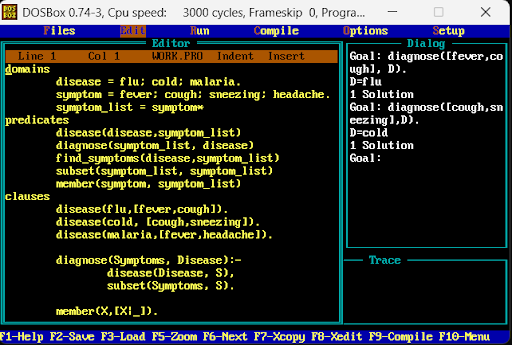
\includegraphics[width=0.8\linewidth]{attachments/medical_expert_sys.png}}
    \caption{Output of \texttt{medicalES.pl}}

\end{figure}

\section{Conclusion}
In this practical, a basic medical expert system was implemented in Prolog using a rule-based knowledge base of diseases and their associated symptoms.
The system successfully performed both forward reasoning and backward reasoning.
\\
\divline
\chapter{Append Two Lists in Prolog}

\section{Problem Statement}
Write a prolog program to append two lists.

\section{Implementation}
\begin{lstlisting}
domains
	List = integer*
predicates
	append_list(list, list, list)
clauses
	append_list([], L, L).
	append_list([H|T], L, [H|R] ) :- append_list(T, L, R)
\end{lstlisting}

\section{Output}
\begin{lstlisting}
# OUTPUT
Goal: append_list([1,2,3],[4,5,6],X)
X = [1,2,3,4,5,6]
1 Solution
\end{lstlisting}

\begin{figure}[H]
    \centering
    \fbox{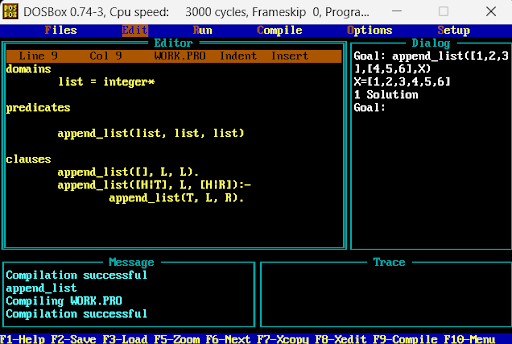
\includegraphics[width=0.8\linewidth]{attachments/append_two_lists.png}}
    \caption{Output of \texttt{append\_two\_lists.pl}}
\end{figure}

\section{Conclusion}
In this practical, a prolog program to append two lists was implemented succesfully.
\\
\divline

\chapter{Reverse a List in Prolog}

\section{Problem Statement}
Write a prolog program to reverse a list.

\section{Implementation}
\begin{lstlisting}
domains
	List = symbol*

predicates
	append(list, list, list)
	reverse_list(list, list)

clauses
    append([], List, List)
    append([H|T], List2, [H|List3]):-
    append(T, List2, List3).
    reverse_list([], []).
    reverse_list([H|T], Rev):-	reverse_list(T, RevT),
    append(RevT, [H], Rev).
\end{lstlisting}

\section{Output}
\begin{lstlisting}
# OUTPUT
Goal: reverse_list([1,2,3],R)
R = [3,2,1]
1 Solution

Goal: reverse_list([a,b,c,d],R)
R = [d,c,b,a]
1 Solution
\end{lstlisting}

\begin{figure}[H]
\centering
\fbox{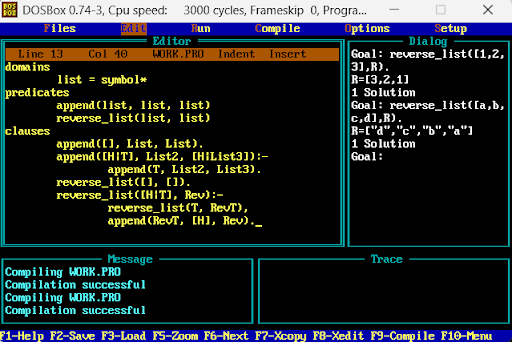
\includegraphics[width=0.8\linewidth]{attachments/reverse_list.png}}
\caption{Output of \texttt{reverse\_list.pl}}
\end{figure}

\section{Conclusion}
In this practical, a prolog program to reverse a list was successfully implemented.
\\
\divline

\chapter{Finding $n^{th}$ Element in Prolog}

\section{Problem Statement}
Write a program to remove the nth element from the list in Prolog.

\section{Implementation}
\begin{lstlisting}
domains
    list = integer*

predicates
    nth_element(integer, list, integer)

clauses
    nth_element(1, [H|_], H).
    nth_element(N, [_|T], X) :-
        N > 1,
        N1 = N - 1,
        nth_element(N1, T, X).
\end{lstlisting}

\section{Output}
\begin{lstlisting}
# OUTPUT
nth_element(2,[10,20,30],X)
X = 20
1 Solution

nth_element(3,[1,2,3,4,5],X)
X = 3
1 Solution
\end{lstlisting}

\begin{figure}[H]
\centering
\fbox{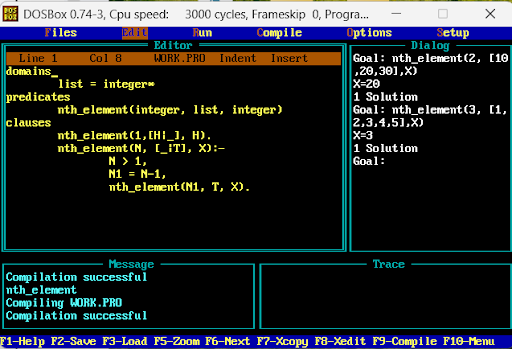
\includegraphics[width=0.8\linewidth]{attachments/nth_element.png}}
\caption{Output of \texttt{remove\_nth\_element.pl}}
\end{figure}
\section{Conclusion}
In this practical, a prolog program to remove the $n^{th}$ element from the list was implemented
successfully.
\\
\divline

\chapter{Member Check Program in Prolog}
\section{Problem Statement}
Write a prolog program to check whether a given element is a member of a list or not.

\section{Implementation}
\begin{lstlisting}
domains
    list = integer*

predicates
    member(integer, list)

clauses
    member(X, [X|_]).
    member(X, [_|T]) :-
    member(X, T).
\end{lstlisting}

\section{Output}
\begin{lstlisting}
# OUTPUT
member(20, [10,20,30])
	Yes

member(10, [20,30,40])
	No
\end{lstlisting}

\begin{figure}[H]
\centering
\fbox{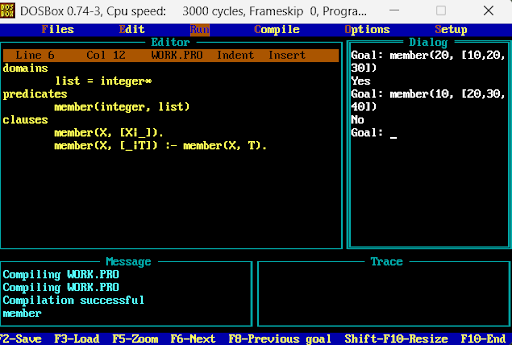
\includegraphics[width=0.8\linewidth]{attachments/member_check.png}}
\caption{Output of \texttt{member\_check.pl}}
\end{figure}

\section{Conclusion}
In this practical, a prolog program to check whether a given element is a member of a list was
implemented successfully.
\\
\divline

\chapter{Fibonacci Series}
\section{Problem Statement}
Implement a program to generate the Fibonacci series upto a given number $N$ in Prolog.

\section{Implementation}
\begin{lstlisting}
domains
    num = integer

predicates
    fibonacci(num, num)

clauses
    fibonacci(0, 0).
    fibonacci(1, 1).
    fibonacci(N, F) :-
    N > 1,
            N1 = N - 1,
            N2 = N - 2,
            fibonacci(N1, F1),
            fibonacci(N2, F2),
            F = F1 + F2.
\end{lstlisting}

\section{Output}
\begin{lstlisting}
# OUTPUT
fibonacci(6,X)
	X = 8

fibonacci(10,x)
    X = 55
\end{lstlisting}
\begin{figure}[H]
    \centering
    \fbox{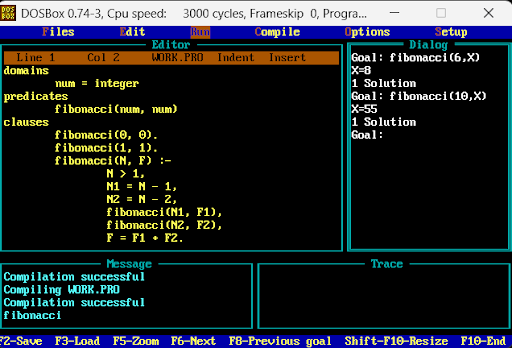
\includegraphics[width=0.8\linewidth]{attachments/fibonacci.png}}
    \caption{Output of \texttt{fibonacci.pl}}
\end{figure}

\section{Conclusion}
In this practical, a prolog program to generate the fibonacci series upto a given number $N$
was successfully implemented.
\\
\divline

\chapter{Factorial Series}
\section{Problem Statement}
Implement a program to display the Factorial of a given number $N$ in Prolog.

\section{Implementation}
\begin{lstlisting}
domains
    num = integer

predicates
    factorial(num, num)

clauses
    factorial(0, 1).
    factorial(N, F) :-
            N > 0,
            N1 = N - 1,
            factorial(N1, F1),
            F = N * F1.
\end{lstlisting}

\section{Output}
\begin{lstlisting}
# OUTPUT
factorial(5, X)
	X = 120
	1 Solution

	factorial(3, X)
	X = 6
	1 Solution
\end{lstlisting}

\begin{figure}[H]
    \centering
    \fbox{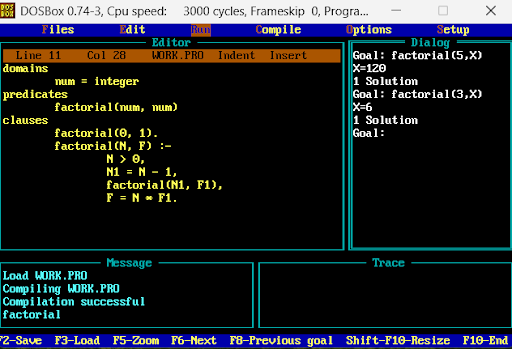
\includegraphics[width=0.8\linewidth]{attachments/factorial.png}}
    \caption{Output of \texttt{factorial.pl}}
\end{figure}

\section{Conclusion}
In this practical, a prolog program to display the factorial of a given number $N$ was successfully
implemented.
\\
\divline
\chapter{Tower of Hanoi}

\section{Problem Statement}
Implement a program to solve the tower of hanoi in Prolog.

\section{Theory}
The \textbf{Tower of Hanoi} is a classical recursive problem in computer science and mathematics. It consists of three pegs and a set of disks of distinct sizes, initially stacked in ascending order of size on the source peg (largest at the bottom, smallest at the top). The objective is to move the entire stack to a destination peg, obeying the following rules:

\begin{enumerate}
    \item Only one disk may be moved at a time.
    \item Each move consists of taking the topmost disk from one peg and placing it on another peg.
    \item A larger disk may never be placed on top of a smaller disk.
\end{enumerate}

\subsection{Recursive Structure}

The problem has a naturally recursive structure. To move $N$ disks from peg $A$ to peg $C$ using peg $B$ as auxiliary:

\begin{enumerate}
    \item Recursively move $N-1$ disks from $A$ to $B$ (using $C$ as auxiliary).
    \item Move the largest disk directly from $A$ to $C$.
    \item Recursively move $N-1$ disks from $B$ to $C$ (using $A$ as auxiliary).
\end{enumerate}

The base case is $N = 1$: simply move the single disk from the source peg to the destination peg directly.
\subsection{Problem Characteristics}
\begin{enumerate}
    \item The problem is defined recursively, solving for $N$ disks reduces to two subproblems of $N-1$ disks.
    \item The number of moves grows as $2^N - 1$, making it computationally expensive for large $N$.
    \item The total number of distinct states is $3^N$, since each of the $N$ disks can be on any of the 3 pegs at any point.
    \item The problem maps directly to logical rules, making it expressible cleanly in Prolog without procedural control flow.
\end{enumerate}

\subsection{Allowed Operations}
\begin{table}[H]
\centering
\begin{tabular}{ll}
\toprule
\textbf{Operation} & \textbf{Description} \\
\midrule
Move disk from Source to Auxiliary  & Place smallest available disk from Source onto Auxiliary \\
Move disk from Source to Target     & Place smallest available disk from Source onto Target \\
Move disk from Auxiliary to Source  & Place smallest available disk from Auxiliary onto Source \\
Move disk from Auxiliary to Target  & Place smallest available disk from Auxiliary onto Target \\
Move disk from Target to Source     & Place smallest available disk from Target onto Source \\
Move disk from Target to Auxiliary  & Place smallest available disk from Target onto Auxiliary \\
\bottomrule
\end{tabular}
\caption{Allowed operations in the Tower of Hanoi Problem}
\end{table}

\section{Implementation}
\begin{lstlisting}
domains
    num = integer
    peg = symbol

predicates
    hanoi(num, peg, peg, peg)

clauses
    hanoi(1, A, _, C) :-
    write("Move disk from "), write(A),
    write(" to "), write(C), nl.
    hanoi(N, A, B, C) :-
            N > 1,
            N1 = N - 1,
            hanoi(N1, A, C, B),
            hanoi(1, A, B, C),
            hanoi(N1, B, A, C).
\end{lstlisting}

\section{Output}
\begin{lstlisting}
hanoi(3, a, b, c)
	Move disk from a to c
	Move disk from a to b
	Move disk from c to b
	Move disk from a to c
	Move disk from b to a
	Move disk from b to c
	Move disk from a to c
	Yes
\end{lstlisting}

\begin{figure}[H]
    \centering
    \fbox{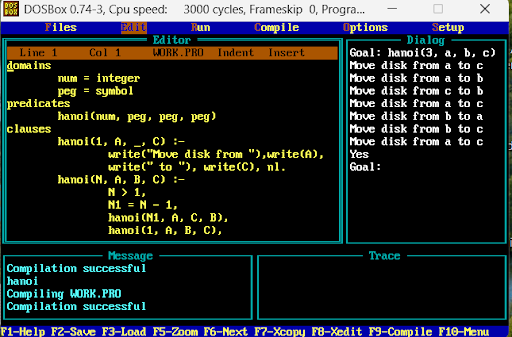
\includegraphics[width=0.8\linewidth]{attachments/hanoi.png}}
    \caption{Output of \texttt{tower\_of\_hanoi.pl}}
\end{figure}

\section{Conclusion}
In this practical, the tower of hanoi problem was successfully solved in Prolog.
\\
\divline

\chapter{Tic-Tac-Toe using Minimax}

\section{Problem Statement}
Implement the Tic-Tac-Toe game using the Mini-max algorithm for adversarial search. \\\\
\textcolor{gray}{(Note: The first move is to be made by humans. The next move should be made by the computer and so on.)}

\section{Theory}
\subsection{Adversarial Search}
In single-agent search, you control every action. The environment responds deterministically to an action. The agent either tries to minimize cost or maximize profit.

In adversarial search, the environment includes other agents whose goal is the inverse of yours. Therefore, every plan you make must account for the fact that the opponent will try to defeat it.

This transforms the problem from finding the best path  finding the best strategy assuming that the opponent plays optimally (requiring a different way to reason about the solution).

\begin{definition}
    Adversarial Search is a branch of artificial intelligence concerned with decision making in competitive
    and \textbf{multi-agent environments}, specifically where two or more agents have conflicting goals.
\end{definition}

It's a class of search problems where two agents act in opposition, each trying to maximize their own
outcome while minimizing the opponent's outcome.

\subsection{Minimax Algorithm}
It's an algorithm that constructs a complete game tree from the current state.
\begin{definition}
Minimax is a recursive, depth-first search algorithm that computes the optimal move for MAX assuming
both players play perfectly.
\end{definition}
It assigns a utility value to each terminal state and propagates these values through the tree.
MAX nodes take the maximum of their children's values, MIN nodes take the minimum.
The root's best child is the move the computer makes.

Formally,
$$
\text{minimax}(n) =
\begin{cases}
\text{utility}(n) & \text{if } n \text{ is a terminal node} \\
\max\limits_{c \in \text{children}(n)} \text{minimax}(c) & \text{if } n \text{ is a MAX node} \\
\min\limits_{c \in \text{children}(n)} \text{minimax}(c) & \text{if } n \text{ is a MIN node}
\end{cases}
$$
Key properties of the minimax algorithm include:
\begin{itemize}
\item It's complete, i.e, finds a move if one exists.
\item It's optimial, i.e, plays perfectly against a perfect opponent.
\item $O^{b^{m}}$ where $b$ is the branching factor.
\end{itemize}

\subsection{Problem Characteristics}
Tic-Tac-Toe has the following characteristics:
\begin{itemize}
    \item It's a two-player, \textbf{zero sum}, perfect-information game.
    \item The state space is finite: $9! = 362880$ possible arrangements.
    \item The game is guaranteed to terminate within 9 moves.
    \item Minimax always finds the optimal move and perfect play from both sides results in a draw.
\end{itemize}

\subsection{Allowed Operations}
\begin{table}[H]
\centering
\begin{tabular}{ll}
\toprule
\textbf{Operation} & \textbf{Description} \\
\midrule
Place mark on empty cell & Current player places X or O on any unoccupied cell \\
Check row win           & Three identical marks occupy any complete row \\
Check column win        & Three identical marks occupy any complete column \\
Check diagonal win      & Three identical marks occupy either diagonal \\
Check draw              & All 9 cells filled with no winning combination \\
Switch player           & Turn passes from X to O or O to X after each move \\
\bottomrule
\end{tabular}
\caption{Allowed operations in the Tic-Tac-Toe Problem}
\end{table}
\newpage
\section{Implementation}
\begin{lstlisting}
import math

HUMAN = 'X'
COMPUTER = 'O'
EMPTY = ' '

def print_board(board):
    for i in range(3):
        print(board[i*3], board[i*3+1], board[i*3+2])

def check_winner(board, player):
    wins = [
        [0,1,2],[3,4,5],[6,7,8],
        [0,3,6],[1,4,7],[2,5,8],
        [0,4,8],[2,4,6]
    ]
    return any(all(board[c] == player for c in line) for line in wins)

def get_empty_cells(board):
    return [i for i, cell in enumerate(board) if cell == EMPTY]

def is_terminal(board):
    return check_winner(board, HUMAN) or check_winner(board, COMPUTER) or not get_empty_cells(board)

def minimax(board, is_maximising):
    if check_winner(board, COMPUTER): return 1
    if check_winner(board, HUMAN): return -1
    if not get_empty_cells(board): return 0
    if is_maximising:
        best = -math.inf
        for cell in get_empty_cells(board):
            board[cell] = COMPUTER
            best = max(best, minimax(board, False))
            board[cell] = EMPTY
        return best
    else:
        best = math.inf
        for cell in get_empty_cells(board):
            board[cell] = HUMAN
            best = min(best, minimax(board, True))
            board[cell] = EMPTY
        return best

def computer_move(board):
    best_score = -math.inf
    best_cell = None
    for cell in get_empty_cells(board):
        board[cell] = COMPUTER
        score = minimax(board, False)
        board[cell] = EMPTY
        if score > best_score:
            best_score = score
            best_cell = cell
    board[best_cell] = COMPUTER

def human_move(board):
    while True:
        try:
            move = int(input("move (1-9): ")) - 1
            if move in get_empty_cells(board):
                board[move] = HUMAN
                break
        except ValueError:
            pass

def play():
    board = [EMPTY] * 9
    for turn in range(9):
        if is_terminal(board): break
        human_move(board) if turn % 2 == 0 else computer_move(board)
        print_board(board)
    if check_winner(board, HUMAN): print("you win")
    elif check_winner(board, COMPUTER): print("computer wins")
    else: print("draw")

if __name__ == '__main__':
    play()
\end{lstlisting}

\section{Output}
\begin{figure}[H]
    \centering
    \fbox{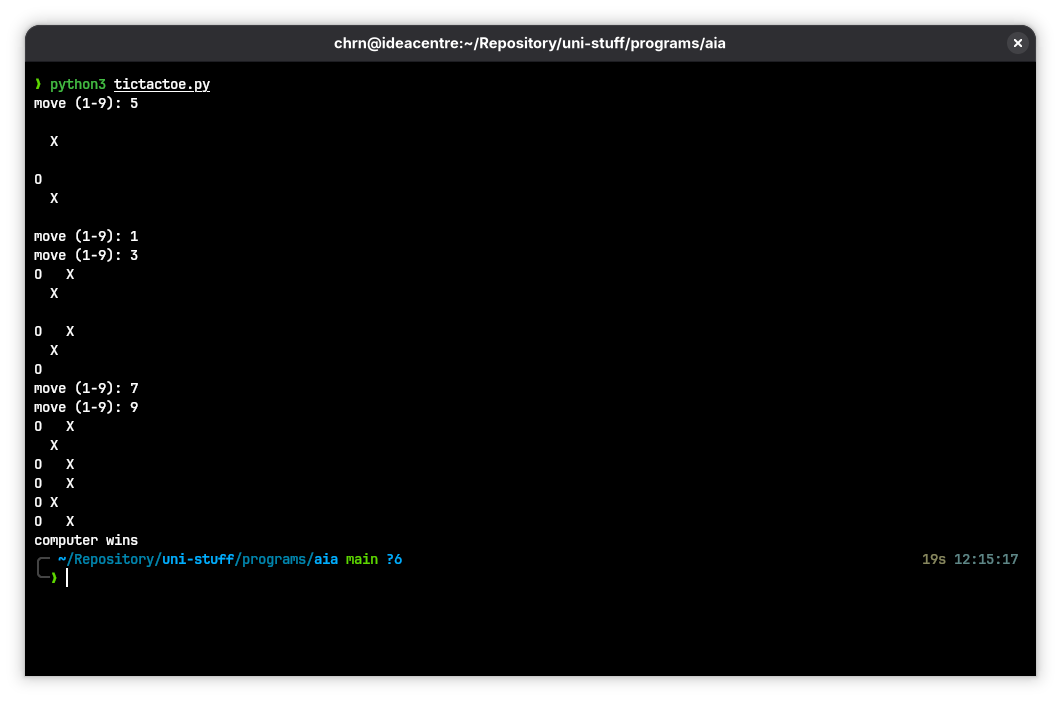
\includegraphics[width=0.8\linewidth]{attachments/tictactoe.png}}
    \caption{Output of the Tic-Tac-Toe python program}
\end{figure}

\section{Conclusion}
In this practical, TicTacToe was successfully implemented using the Minimax algorithm for
adversarial search. The computer always plays the optimal move, making it impossible for a human
to win. If a human plays perfectly then the result is always a draw.
\\
\divline
\chapter{Eliza and ChatGPT Dialogues}
\section{Problem Statement}
Perform the following:
\begin{enumerate}
\item Get an intelligent dialogue out of \textbf{ELIZA}
\item Get an intelligent dialogue out of \textbf{ChatGPT}
\end{enumerate}

\section{Model Comparison}
\begin{table}[h]
\centering
\begin{tabular}{lll}
\toprule
\textbf{Feature} & \textbf{ELIZA} & \textbf{ChatGPT} \\
\midrule
Mechanism & Pattern matching & Neural LLM (transformer) \\
Knowledge & None (script only) & Broad world knowledge \\
Context memory & None & Multi-turn context window \\
Year & 1966 & 2022 \\
Responses & Reflective questions & Generative answers \\
\bottomrule
\end{tabular}
\caption{Comparison of ELIZA and ChatGPT}
\end{table}

\section{Conversations}
\subsection{ELIZA Dialogue}

\begin{dialogue}
\speak{User} I am feeling very anxious lately.
\speak{ELIZA} \texttt{Why do you say you are feeling very anxious lately?}
\speak{User} I think it's because of my exams.
\speak{ELIZA} \texttt{Do you often think it's because of your exams?}
\speak{User} Yes, I always feel nervous before exams.
\speak{ELIZA} \texttt{Can you think of a specific example?}
\speak{User} Last week I couldn't sleep the night before my test.
\speak{ELIZA} \texttt{Tell me more about that.}
\end{dialogue}

\subsection{ChatGPT Dialogue}

\begin{dialogue}
\speak{User} Explain the difference between supervised and unsupervised learning.
\speak{ChatGPT} \texttt{Supervised learning uses labelled data --- each training example has an input
and a known output, and the model learns to map inputs to outputs. Examples include
classification and regression. Unsupervised learning works on unlabelled data and tries
to find hidden structure --- examples include clustering (K-Means) and dimensionality
reduction (PCA). The key difference is whether ground-truth labels are available during training.}
\speak{User} Which one would you use for customer segmentation?
\speak{ChatGPT} \texttt{Customer segmentation is typically done with unsupervised learning,
specifically clustering algorithms like K-Means or DBSCAN, since you don't have predefined
labels for which segment a customer belongs to. The algorithm groups customers by similarity
in behaviour, demographics, or purchase history.}
\end{dialogue}

\section{Conclusion}
In this practical, intelligent dialogues were obtained from both ELIZA and ChatGPT. ELIZA simulates conversation purely through pattern matching and keyword substitution
with no understanding of meaning, while ChatGPT generates contextually coherent responses.
\\
\divline
\chapter{Link Grammar Parser}

\section{Problem Statement}
Parse English sentences using the Link Grammar Parser.
\section{Theory}
Link Grammar is a syntactic formalism developed by Davy Sleator and Davy Temperley at Carnegie Mellon University in 1991. Unlike phrase-structure grammars that build hierarchical parse trees, Link Grammar describes sentence structure through direct binary relationships between words, called \textit{links}.

\begin{definition}
A \textbf{Link Grammar} is a formal grammar in which each word in a sentence is associated with a set of \textit{connector requirements}. A sentence is grammatically valid if and only if all connector requirements of every word are simultaneously satisfied by non-crossing links between word pairs.
\end{definition}

\begin{definition}
A \textbf{link} is a labeled, undirected binary connection between two words in a sentence. Each link type encodes a specific syntactic relationship, such as subject-verb (\texttt{S}), verb-object (\texttt{O}), or determiner-noun (\texttt{D}).
\end{definition}

\begin{definition}
A \textbf{linkage} is a complete and valid assignment of links across all words in a sentence such that every connector requirement is satisfied and no two links cross each other (the planarity constraint).
\end{definition}

\begin{definition}
A \textbf{disjunct} is a specific combination of connectors associated with a word that represents one possible syntactic role that word may play in a sentence. The word dictionary stores all valid disjuncts for each word.
\end{definition}

The parser works by selecting one disjunct per word and attempting to satisfy all connector requirements simultaneously. If multiple valid linkages exist, they are ranked by a cost metric and returned in order of preference.
\subsection{Problem Characteristics}
Link Grammar parsing problem has the following characteristics:
\begin{enumerate}
    \item The grammar is lexicalised: all syntactic information is stored in the word dictionary, not in phrase-structure rules
    \item Parsing is constraint satisfaction: a sentence is valid only if all connector requirements of every word are simultaneously satisfied
    \item The planarity constraint (links must not cross) keeps the search space tractable
    \item Ambiguity is handled naturally: multiple valid linkages can be returned for a single sentence, ranked by a cost metric
    \item The state space grows with sentence length but is bounded by the number of disjuncts in each word's dictionary entry
\end{enumerate}

\section{Implementation}
\subsection{Dependencies}
Install a built-in \texttt{link-grammer} CLI tool for your operating system to parse any input text.
\begin{lstlisting}
# for arch-linux do:
sudo pacman -S link-grammar
\end{lstlisting}

\subsection{Source Code}
This practical has been implemented using the Python programming language.
\begin{lstlisting}
import subprocess

sentences = [
    "The dog chased the ball quickly.",
    "Birds fly south in winter."
]

for sentence in sentences:
    print(f"\nSentence: {sentence}")
    print("-" * 50)
    result = subprocess.run(
        ["link-parser"],
        input=sentence + "\n!quit\n",
        capture_output=True,
        text=True
    )
    print(result.stdout)
\end{lstlisting}

\section{Output}
\begin{figure}[H]
    \centering
    \fbox{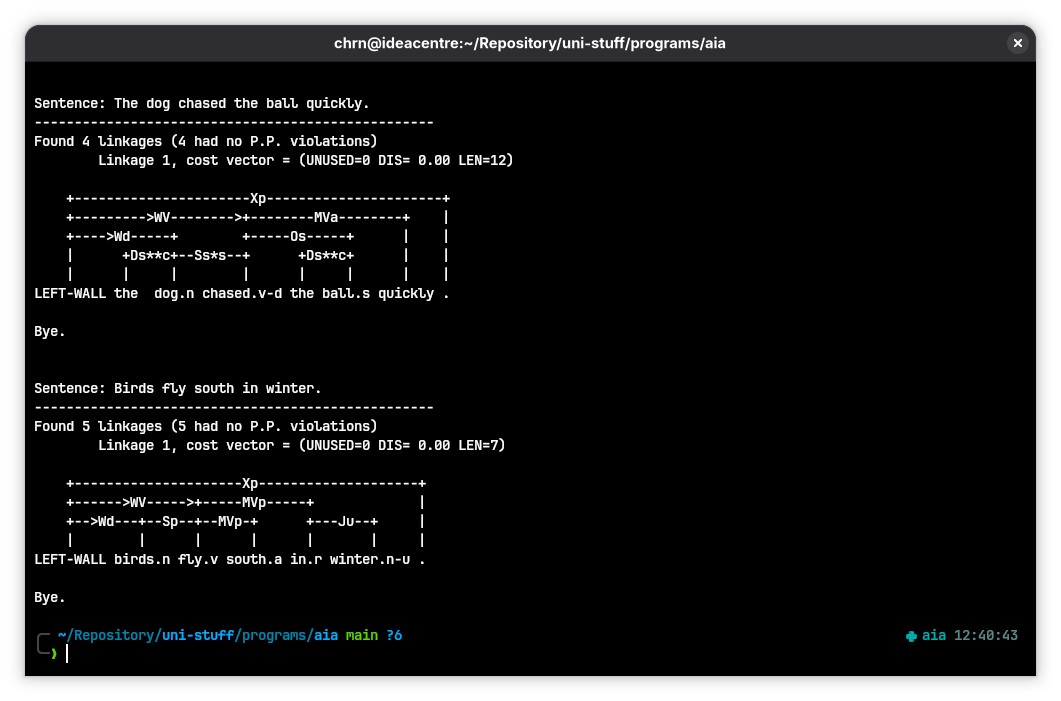
\includegraphics[width=0.9\linewidth]{attachments/link_grammar.png}}
    \caption{Output of the Link Grammar Parser}
\end{figure}

\section{Conclusion}
In this practical, English sentences were successfully parsed using the Link Grammar
Parser. The parser identified syntactic relationships between words using typed links,
demonstrating how Link Grammar represents sentence structure without relying on
phrase-structure rules.
\\
\divline

\chapter{Database Representation in Prolog}
\section{Problem Statement}
Consider a simple database of books and authors:
\begin{itemize}
\item author(jane, book1).
\item author(mary, book2).
\item author(john, book3).
\item author(jane, book4).
\end{itemize}
Perform the following:
\begin{enumerate}
\item Write a Prolog rule to find all books by a given author (including repeated results if the same author wrote multiple books).
\item Write Prolog rule to check if a person is an author. Use cut to prevent unnecessary backtracking.
\end{enumerate}

\section{Implementation}
\begin{lstlisting}
domains
    person, book = symbol

predicates
    author(person, book)
    books_by_author(person, book)
    is_author(person)

clauses
    author(jane, book1).
    author(mary, book2).
    author(john, book3).
    author(jane, book4).

    books_by_author(A, B) :-
        author(A, B).

    is_author(A) :-
        author(A, _), !.
\end{lstlisting}
\section{Output}
\begin{lstlisting}
# OUTPUT
Goal: books_by_author(jane,X).
X=book1
X=book4
2 Solutions

Goals: books_by_author(mary,X).
X=book2
1 Solutions
\end{lstlisting}

\begin{figure}[H]
    \centering
    \fbox{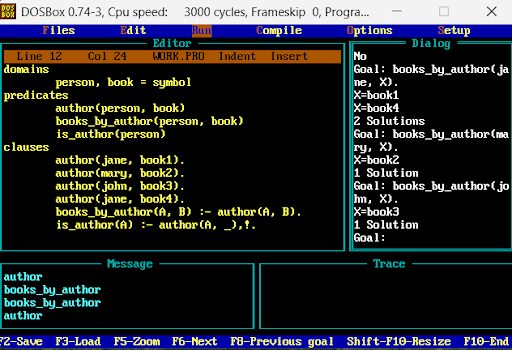
\includegraphics[width=0.6\linewidth]{attachments/prolog_db.png}}
    \caption{Output of \texttt{prolog\_db.pl}}
\end{figure}

\section{Conclusion}
In this practical, we have defined basic logic relations to navigate a database of authors and their works.
The first rule utilizes Prolog's natural backtracking to aggregate multiple results, while the second rule employs the
\textbf{cut operator} ($!$) to efficiently verify a property without redundant searching.
\divline

\chapter{List Member Verification in Prolog}
\section{Problem Statement}
Write a Prolog program to check if a number is a member of a list of integer.
Use cut to prevent backtracking.

\section{Implementation}
\begin{lstlisting}
domains
    list = integer*

predicates
    member_cut(integer, list)

clauses
member_cut(X, [X|_]) :- !.
   member_cut(X, [_|T]) :- member_cut(X, T).
\end{lstlisting}

\section{Output}
\begin{lstlisting}
member_cut(20, [10,20,30])
Yes
member_cut(5, [1,2,3,4,5])
Yes
member_cut(6, [0,2,4])
No
\end{lstlisting}

\begin{figure}[H]
    \centering
    \fbox{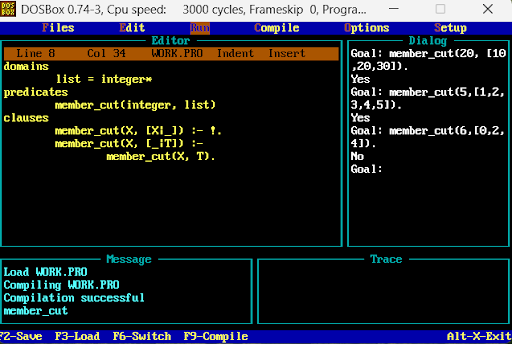
\includegraphics[width=0.8\linewidth]{attachments/member_verification.png}}
    \caption{Output of \texttt{member\_verification.pl}}
\end{figure}

\section{Conclusion}
In this practical, a member list verification program was successfully implemented in Prolog.
\\
\divline
\end{document}
